\chapter{Superscalar Processing}
Superscalar processors rearrange the incoming instruction stream so that instructions can be executed independently across multiple execution units, allowing for increased throughput.

However, in doing so, they must handle parallel decoding, issues that arise from superscalar execution, and must preserve sequential consistency of execution and exception processing.

\section{Parallel Decoding}
In a superscalar machine, multiple instructions are issued concurrently (\autoref{fig:screenshot148}). Decoding these instructions can be difficult, especially when instructions are multiple words. Inter-instruction dependencies need to be checked before an instruction can be issued.

\begin{figure}
\centering
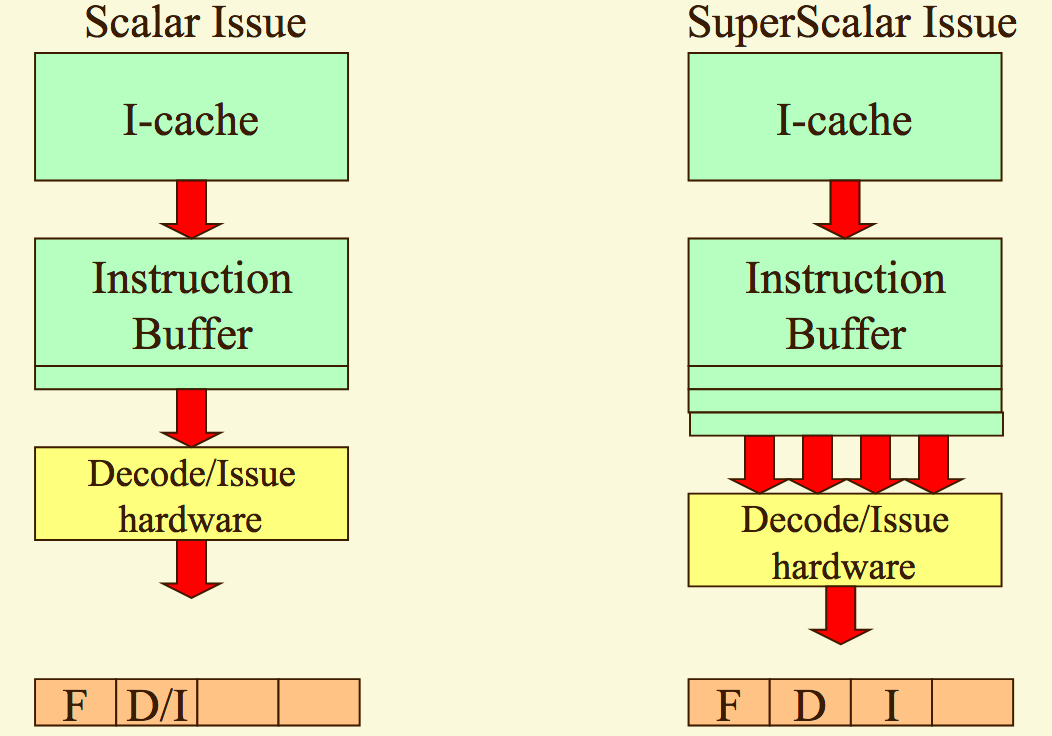
\includegraphics[width=0.7\linewidth]{figures/screenshot148}
\caption{Parallel decoding in a superscalar system.}
\label{fig:screenshot148}
\end{figure}

The decoder is on the critical path of execution, so it must be run. However, CISC (Complex Instruction Set Computer) instructions are hard to decode in parallel, as the length of an instruction is variable (\autoref{fig:screenshot149}); instruction boundaries are normally determined sequentially.

\begin{figure}
\centering
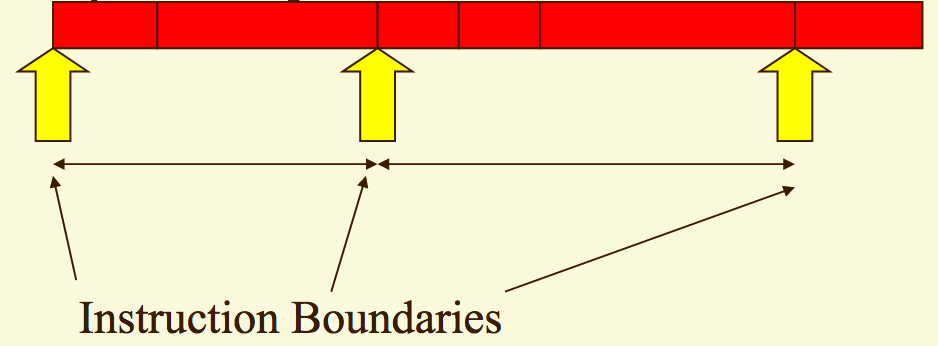
\includegraphics[width=0.7\linewidth]{figures/screenshot149}
\caption{Variable instruction boundaries in a CISC system.}
\label{fig:screenshot149}
\end{figure}

Additionally, register dependencies need to be considered (\autoref{fig:screenshot150}). Sequential issuing of instructions can use ready bits, set during issuing, to detect dependencies; parallel issuing requires combinational logic to determine where dependencies lie.

\begin{figure}
\centering
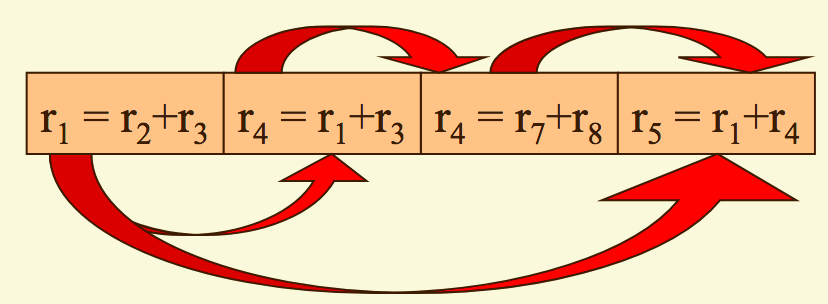
\includegraphics[width=0.7\linewidth]{figures/screenshot150}
\caption{Register dependencies.}
\label{fig:screenshot150}
\end{figure}

The pre-decoding stage is executed differently depending on whether the architecture is RISC (Reduced Instruction Set Computer) or CISC. 

If it is RISC, the instruction class, the type of resources required and sometimes the target address of the branch is required; this may add 4 bits per instruction when the instruction is written into the instruction cache (I-cache). This is shown in \autoref{fig:screenshot151}.

For a CISC system, the instruction boundaries and location of opcodes and operands must be determined; the AMD K5 architecture adds 70\% extra bits to an instruction during the fetching stage.

\begin{figure}
\centering
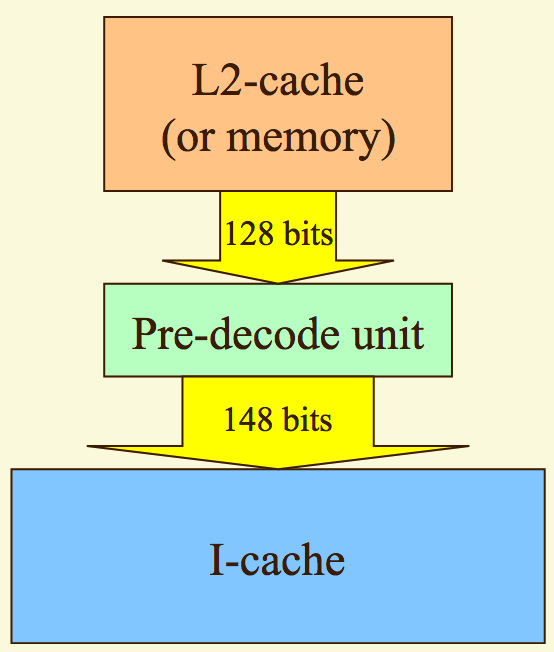
\includegraphics[width=0.7\linewidth]{figures/screenshot151}
\caption{Pre-decode unit adding bits.}
\label{fig:screenshot151}
\end{figure}

\section{Superscalar Instruction Issues}
When evaluating instructions, a variety of issues may arise: \begin{itemize}
\item \textbf{False dependencies}: There may be a false dependency on registers that prevents superscalar execution. This can be resolved using register renaming.
\item \textbf{Unresolved control dependencies}: The next instruction to evaluate may be located after a branch and thus cannot be evaluated until the branch is resolved. This can be resolved by waiting for the result of the branch to be determined, or by speculatively executing the branch and rolling back the result if it is incorrect.
\item \textbf{Use of shelving}: A shelving buffer can be used to execute instructions that do not have dependencies. Essentially, assume you have an instruction stream like the following:
\begin{lstlisting}[language={}]
[1]: load R1, address1 
[2]: load R2, address2
[3]: R3 = R1 + R2
[4]: R4 = R1 / R2
[5]: R5 = R1 - R2
[6]: R6 = R2 + 1
\end{lstlisting}
If the instruction window used to load instructions is three-wide, instructions 1 and 2 will be executed, and instruction 3 will promptly be stalled until 1 and 2 are executed. Assume for some reason that instruction 1, the loading of R1, takes extra time; execution of instructions 3, 4, and 5 will be stalled until R1 is loaded. 

In this case, instructions 3, 4 and 5 are \textit{shelved} until their dependency is resolved, and instruction 6 is executed; this allows for a degree of concurrent processing. This is illustrated in \autoref{fig:screenshot152}. Note that the instructions will now complete out of order, and that the machine will still need to enforce data dependencies and sequential consistency.

\begin{figure}
\centering
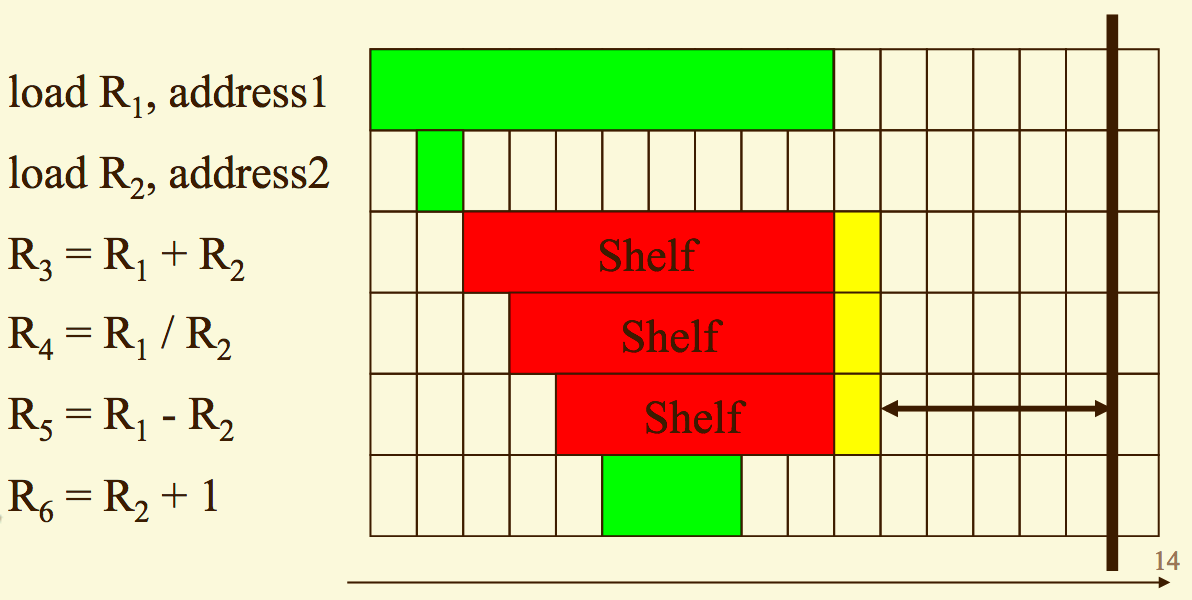
\includegraphics[width=0.7\linewidth]{figures/screenshot152}
\caption{Reducing latency with shelving.}
\label{fig:screenshot152}
\end{figure}

\end{itemize}

When instructions are loaded from the instruction buffer in memory, they go through a Decode/Check issue stage which checks them for dependencies and other issues prior to submission to the execution units. This is handled by a \textit{reservation station}, shown in \autoref{fig:screenshot153}.

\begin{figure}
\centering
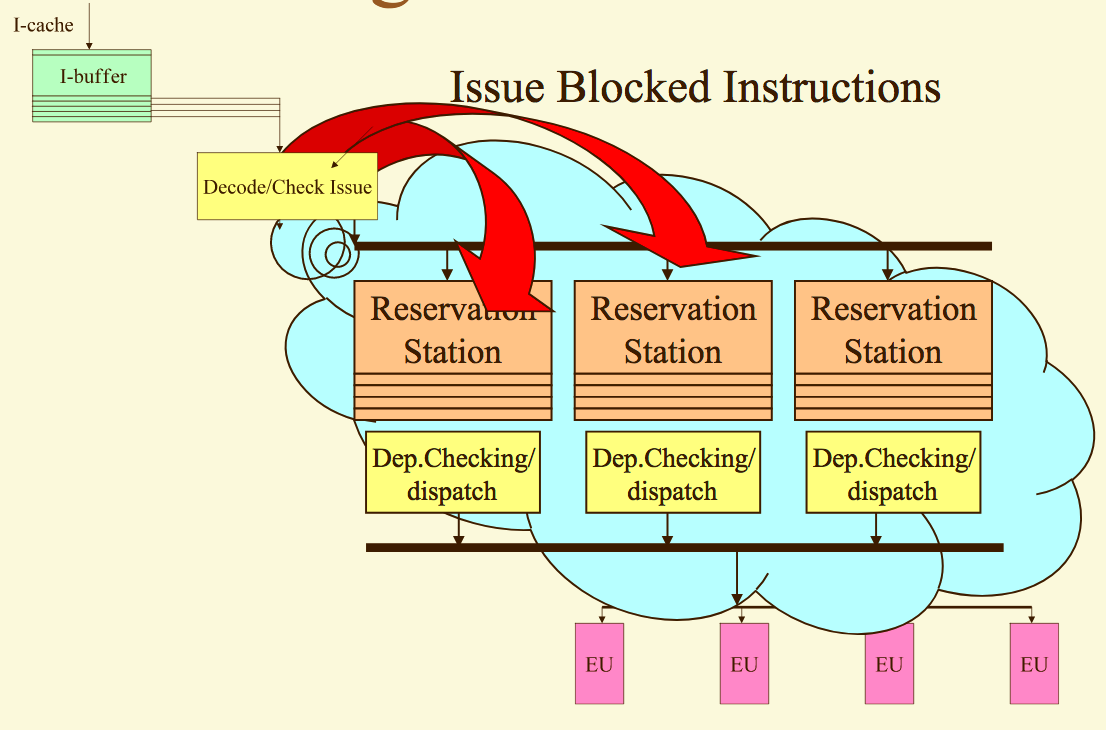
\includegraphics[width=0.7\linewidth]{figures/screenshot153}
\caption{Reservation stations for efficient instruction issue.}
\label{fig:screenshot153}
\end{figure}

\section{Cray-1}
The Cray-1 was an early superscalar machine with different address and scalar functional units. The addressing units had 8 A registers and 64 B registers, while the data registers had 8 S registers and 64 T registers. The B and T registers could be used as program-controlled cache. This is depicted in \autoref{fig:screenshot154}.

\begin{figure}
\centering
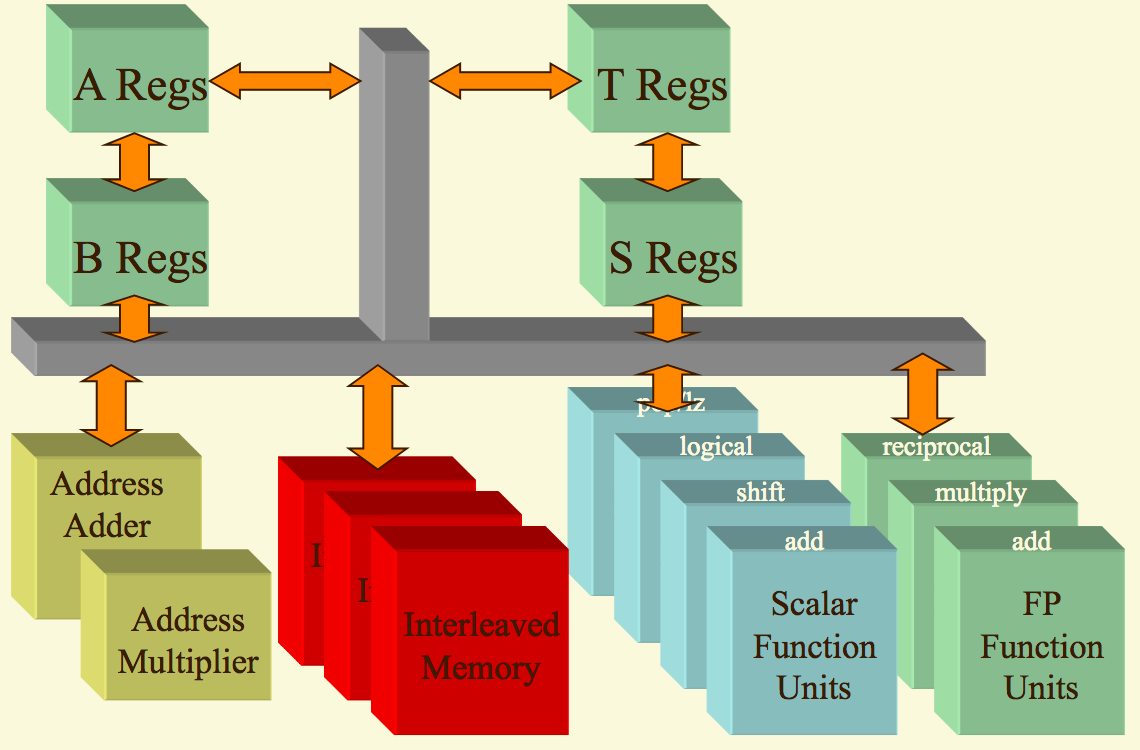
\includegraphics[width=0.7\linewidth]{figures/screenshot154}
\caption{Cray-1 architecture.}
\label{fig:screenshot154}
\end{figure}

The Cray-1 is a register-register oriented machine; the only instructions that interacted with memory were \texttt{load} and \texttt{store}. Instructions that manipulate the B and T registers were restricted to memory access and transfer to the A and S files. Information flow was from memory to the A or S registers, or to the B and T registers. Data for the functional units can only come from the S or A register sets. However, it was possible to conduct block transfers between memory and the B and T register files.

Because there are multiple functional units, it is possible to start the next instruction even if the last one is not complete. The only time this process must freeze is when the next instruction depends on the last one. To resolve this, instructions can be issued out of order; an early scheme developed for this is Tomasulo's algorithm, which was originally developed for the IBM 360/91 floating point unit. 

\section{Tomasulo's Algorithm}
The algorithm attempts to issue instructions even if they cannot be executed; this will prevent them from holding up later instructions. \footnote{If you'd like a nice illustration of how this works, please consult the slides. There's about \textit{forty images} worth.}

Each register is augmented with a Ready bit and a Tag field. Associated with each functional unit is a Reservation Station. Each reservation station can store a pair of operands. Each operand has its own ready bit and tag bit.

A reservation station can also hold a destination tag. When an instruction is issued, a new destination tag is stored into the destination tag field. These destination tags are assigned from a \textit{tag pool}. Instructions are then issued with little regard to data dependencies.

Instructions are issued if the requested functional unit has an available reservation station, there is a free tag available in the tag pool, and a source register can be guaranteed not to be loaded during this cycle. 

When an instruction is issued, the contents of the instruction's source registers, as well as the ready and tag bits of the registers, are copied to the requested functional unit's reservation station. A tag is then allocated from the tag pool and stored in both the reservation station and the tag field of the destination register. The ready bit of the destination register is then cleared.

The crux of Tomasulo's algorithm then applies. If the ready bit in the reservation station is set, the station contains a valid copy of the register's contents. If it is clear, it contains a valid tag; this tag can then be used to find the functional unit responsible for producing the result.

For a functional unit to start execution, all operands must be ready, the unit must not be busy, and it must have access to the bus to return the result to the register file. When an instruction begins execution, it releases the reservation station, reserves the result bus for the appropriate cycle, and attaches the destination tag to the result.

When the result is generated, the tag is compared to all of the tags in all of the reservation stations and all of the registers that have the ready bit clear. The result is stored in all reservation stations that match. The ready bit is then set to indicate that the result is valid, and the tag is returned to the tag pool.

The algorithm supports an unrestricted number of dependent instructions; the tag value is copied to multiple reservation station shelves to accommodate this.

Essentially, this system aims to execute instructions where possible; when instruction execution is not possible - primarily due to a data dependency - the state will be preserved in a reservation station, which will then be loaded with the data when available. This allows concurrent execution of instructions that do not have data dependencies. In doing so, it enforces flow dependence; this is made possible by the fact that tags are assigned to individual instructions, so that two instructions sharing a register in a false dependency can be separated using different tags.

Tomasulo's algorithm also implicitly implements register renaming; different tags are assigned for different instructions, so that false dependencies are implicitly eliminated.

\subsection{Implementation}
Tomasulo's algorithm can be quite hard to implement. Associative hardware is required to support looking for tags in the register file in one clock cycle; additionally, tag allocation and deallocation hardware is required. It provides a deep flow dependence.

\section{Thornton's Algorithm}
Thornton's algorithm is a simpler issue scheme that removes the tags (and thus allocation and deallocation) and the associative hardware on the register files.

The rules for the reservation station are as follows: \begin{itemize}
\item If the ready bit is set, the operand contains data.
\item If the ready bit is clear, the source and destination registers are specified directly.
\end{itemize}

In Thornton's issue scheme, an instruction is issued if the functional unit has some free reservation slots and the destination register is not busy.

When an instruction is issued, a reservation station for the functional unit is reserved. If a source register is ready, then the data is copied to the reservation station and the ready bit is set. If the register is not ready, then the source register number is placed in the SR field and the associated ready bit is cleared. Afterwards, the ready bit for the destination register must be cleared.

Thornton's algorithm will result in more blocks and reduced performance in comparison to Tomasulo's algorithm, but is considerably simpler to implement. The relative performance is shown in \autoref{fig:screenshot155}.

\begin{figure}
\centering
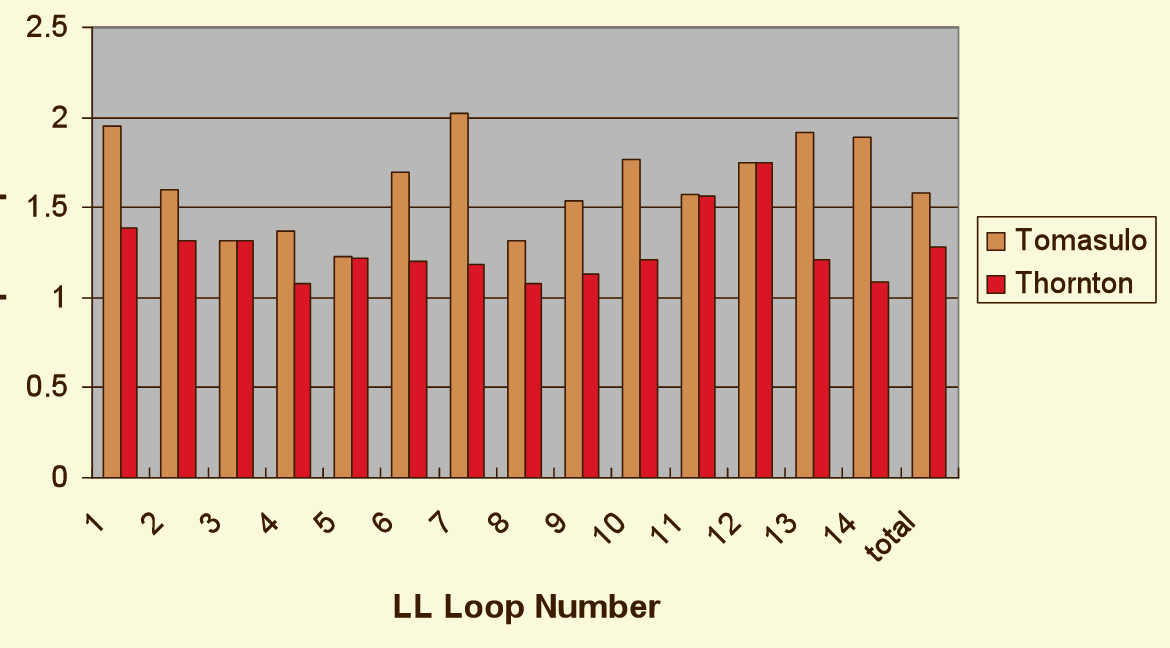
\includegraphics[width=0.7\linewidth]{figures/screenshot155}
\caption{Tomasulo algorithm vs Thornton algorithm.}
\label{fig:screenshot155}
\end{figure}

\section{Other renaming schemes}
The compiler can perform static renaming; however, it cannot account \footnote{The exact wording in the slides was "account account for dynamic variation". I'm not entirely sure if that was meant to be a \textit{can} or a \textit{cannot}, but based on the Levenshtein distance I've opted for the latter.} for dynamic variation in delays. This means that it will have to use more resources to provide "ideal" performance.

The PowerPC renaming scheme uses a separate register rename file, and associative access to the register file. This means that registers used by executing code are not necessarily the real registers; instead, they are dynamically remapped during execution to maximise performance (\autoref{fig:screenshot156}). Operand fetching occurs during renaming. 

\begin{figure}
\centering
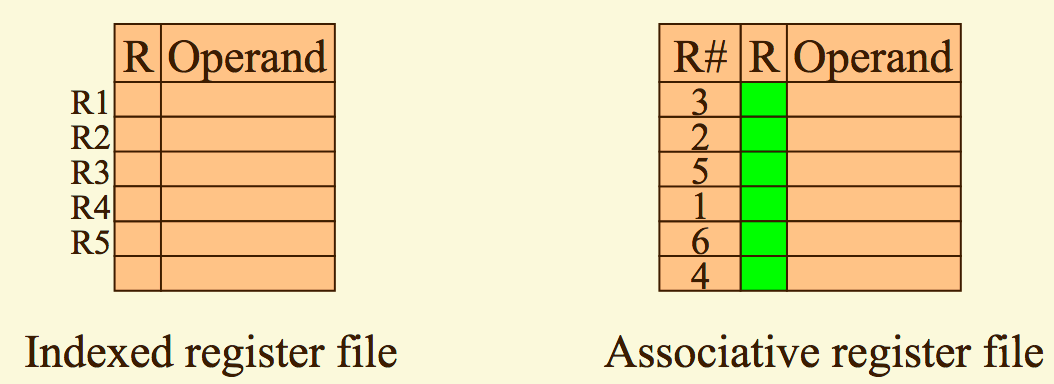
\includegraphics[width=0.7\linewidth]{figures/screenshot156}
\caption{Indexed vs associative register file.}
\label{fig:screenshot156}
\end{figure}

However, there may be more than one version of a particular register in use at any given time; this is resolved by using another bit in the register file, the \textit{latest bit}, to indicate whether a particular register is the latest version or not. Fetches from the register file retrieve the most recent (last) write; outstanding instructions take the index of the most recent register to write to.

\section{Memory data dependence}
The schemes discussed to date only work for register-enforced consistency. If memory access is conducted as part of the instruction stream, is it possible to conclude whether data dependence exists?

\subsection{Static dependence determination}
The compiler can determine when data dependence cannot exist. As an example, $A(i) \gets A(i+1)$ must be a different location, and can thus be treated relatively independently.

\subsection{Dynamic dependence determination}
To resolve the problem dynamically, the hardware must keep track of outstanding stores. This is done by maintaining an associative queue of outstanding operations; when a read is requested, the outstanding queue is searched to determine if a pending store is present (\autoref{fig:screenshot157}). This is easier to implement on a RISC architecture than a CISC architecture.

\begin{figure}
\centering
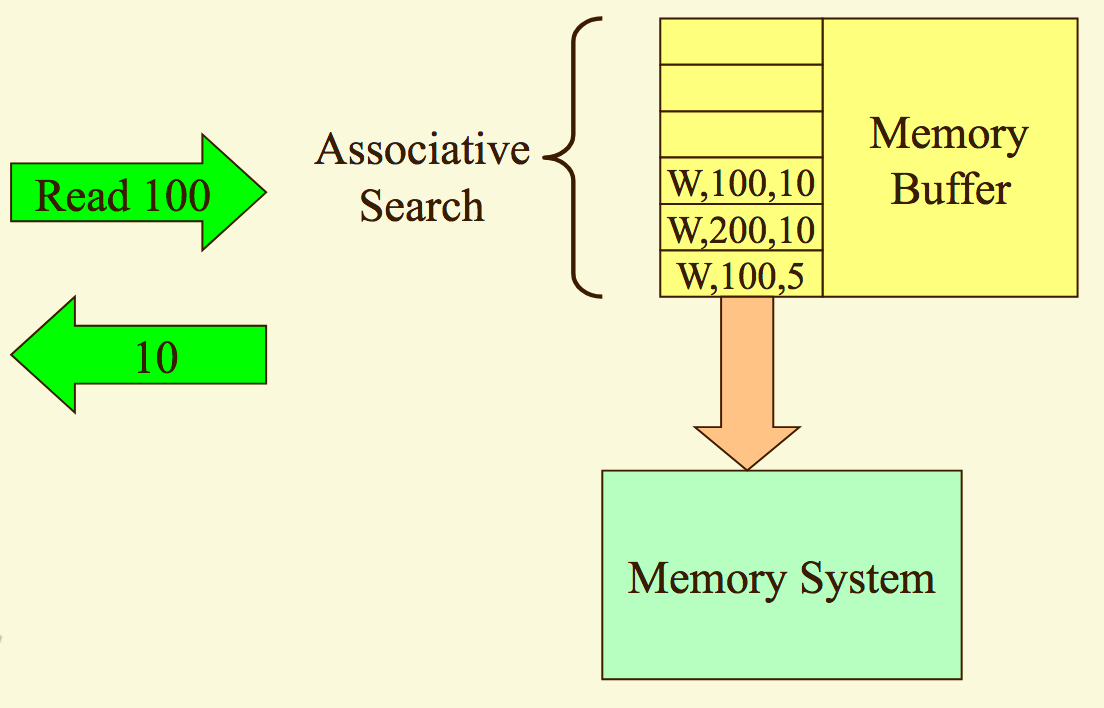
\includegraphics[width=0.7\linewidth]{figures/screenshot157}
\caption[Memory dependence checking.]{Memory dependence checking with an associative queue. $W,100,10$ refers to writing $10$ to the memory location $100$.}
\label{fig:screenshot157}
\end{figure}

\section{Preserving sequential consistency}
Instructions are issued in order, but may complete out of order. This may cause issues with speculative execution and precise interrupts.

\subsection{Precise interrupts}
On a non-pipelined machine in which instructions are executed in order, a hardware interrupt (i.e. an I/O event or a detected fault) can preserve the current instruction pointer and processor state.

However, if the machine is pipelined, the current instruction pointer is significantly less precise, and preservation of processor state may become problematic.

If instructions finish out of order, then the state of the processor is not sequentially consistent. Some later instructions will be completed, and some earlier instructions may not be completed. This makes it difficult to restart the current instruction flow if recovery is required (e.g. in the case of a page fault). Additionally, debugging information may be incorrect.

If precise interrupts are required, a reorder buffer can be used to enforce in-order completion. Instructions can still be issued even if they are blocked; subsequence instructions can still execute out of order, but they must complete in-order. This is shown in \autoref{fig:screenshot158}.

\begin{figure}
\centering
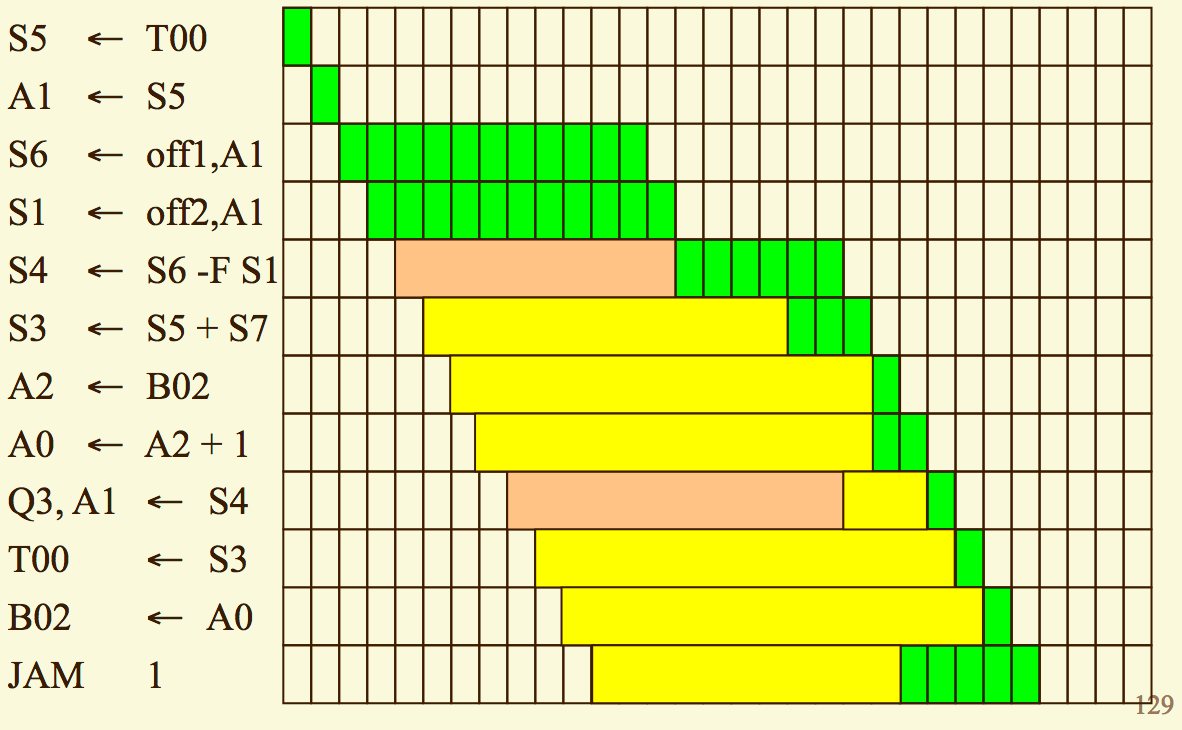
\includegraphics[width=0.7\linewidth]{figures/screenshot158}
\caption[In-order completion.]{In-order completion; out-of-order execution is purposely stalled to ensure that instructions complete in order.}
\label{fig:screenshot158}
\end{figure}

The reorder buffer is implemented using a circular buffer with head and tail pointers (\autoref{fig:screenshot159}). The instructions are written to the reorder buffer in strict program order. Each instruction can be in one of three states: issued, in execution and finished. An instruction is only allowed to retire if it is finished and all previous instructions are retired.

\begin{figure}
\centering
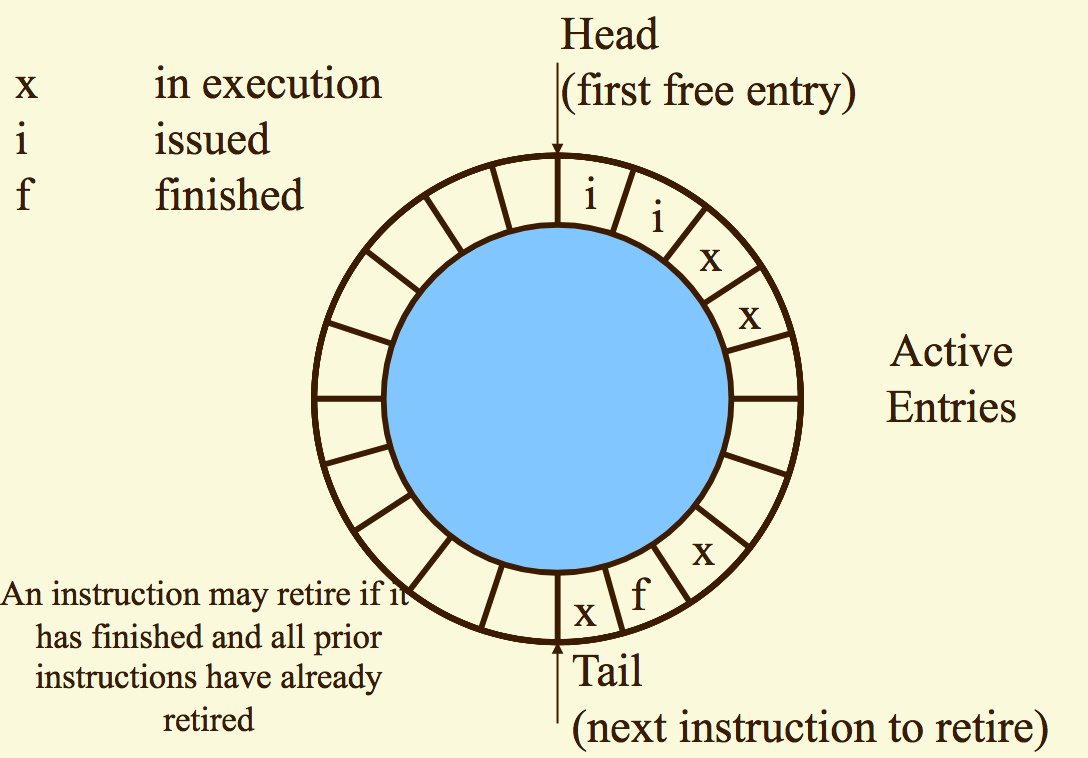
\includegraphics[width=0.7\linewidth]{figures/screenshot159}
\caption{Reorder buffer implementation.}
\label{fig:screenshot159}
\end{figure}


